%% \documentclass[a4paper]{article}
\documentclass[12pt]{article}

%% Language and font encoding
\usepackage[english]{babel}
\usepackage[utf8x]{inputenc}
\usepackage[T1]{fontenc}

\usepackage{tgtermes} % times font

%% Sets page size and margins
\usepackage[a4paper,top=3cm,bottom=2cm,left=3cm,right=3cm,marginparwidth=1.75cm]{geometry}

%% Useful packages
\usepackage{amsmath}
\usepackage{graphicx}
\usepackage[colorinlistoftodos]{todonotes}
\usepackage[colorlinks=true, allcolors=blue]{hyperref}
\usepackage[useregional]{datetime2}
\usepackage{array}
\usepackage{tabularx}
\usepackage{natbib}
\usepackage{authblk}
\usepackage{enumitem}
\usepackage{setspace}
\usepackage{enumitem}


\renewcommand{\baselinestretch}{1.5} 






\title{Evaluation of Community Detection Algorithm}
\author{Ping-Chang Lee}
\affil{MSc in Data Science \& Statistics \\ The University of Bath}
\date{{September}{2022}}

\begin{document}
\maketitle
\pagebreak

%% Access Page 1
    
\bigbreak\bigbreak\bigbreak
\bigbreak\bigbreak\bigbreak
\bigbreak\bigbreak\bigbreak

This dissertation may be made available for consultation within the University Library and may be photocopied or lent to other libraries for the purposes of consultation.
\bigbreak\bigbreak\bigbreak
Singed: ***My Signature Here***
\pagebreak


\tableofcontents
\pagebreak

\section{Introduction}
When researchers conducting analysis on their topics, while processing data, the format of data can be form in various fashion. Table is perhaps one of the most commonly used format for data storage. However, it can be arduous for researchers to observe the relation between rows(or columns) if the data is in large scale. To ease the pain, network structure is an excellent data format that is popular among the researchers if they would like to focus on analysing data structure-wise. For analysis that is related to network structure such as study how the network change over time, visualizing the complex network, and the topic that is related to this dissertation, detecting communities within network, are called network analysis. In recent decades, the study related to network analysis has drawn the attention of scholars form various fields. Among numerous topics of network analysis, discovering the community structure of network is one of the most essential approach to learn the complicated systems that can not easily be cracked by solely conducting shallow researches\cite{1}. 

%% Add motivation/ The brief intro of the dissertation.
\bigbreak

Despite there are dozens of community detection algorithms already implemented to real-world network analysis and have already granted great success in many fields \cite{2,3}, the sample networks for performance testing are often simplified and sparse. In this dissertation, the LFR benchmark graph is introduced to mock the real-world network by increasing the complexity of the network. Afterwards, a subset of community detection algorithms are applied to the artificial network. Due to the nature of algorithms, the dissertation will introduce the computation complexity and their procedures. Also, since some algorithms are iterative, the dissertation selects the best result from iterations for evaluations under different circumstances. Next, the dissertation provides a series of approaches to evaluate the partitions of algorithms. As mentioned, a network can have either high complexity or very sparse structure, there is no consistent classification yet to determine if a given partition of a network is 'good'. The dissertation particularly underline the methodology on goodness of partition and the measure of similarity between the partition of a community detection algorithm and the ground truth community partition(network that is already labeled by communities).

\section{Background}

%% Rephrase this. 
In this section, the dissertation introduces the background knowledge for this dissertation, that is, network and community. In subsection 2.1, introduction to network structure, the basic terms used in both network analysis is firstly introduced. Secondly, in order to better understand the impact of data structures on community detection algorithms with respect to computational complexity, three of the most commonly used abstract data type for network data storage is also explained with examples. The next subsection, community, establishes the basic representation of community structure initially; afterwards, types of community are address accordingly.

\subsection{Network Structure}

The two smallest elements in network structure are vertex and edge, denoted as $v$ and $e$. Vertex is simply a node within the network, and a vertex(or a node) can contain multiple information. For instance, in social network study, each vertex represents a user, and therefore may contain some information such as phone number, physical address, searching preference, and so on.  Therefore, vertex can be treated as atom within a particle, even though vertex can take a collection of information, yet is not divisible, meaning can not be broken into smaller vertices by default. The other element is edge, an edge represent the connection between two vertices within the same network. The definition of edge is as follows:  There is an edge between vertex $v_i$ and vertex $v_j$, where $v_i$ and $v_j$ both belong to network(or a graph) $G$, if there exists an connection(or relation) between $v_i$ and $v_j$. One thing worth noticing is that an edge can be directed or weighted. For networks that contains weighted edges, the network is called weighted network; similarly, for networks that contains undirected edges, the network is called directed network. A great example of directed and weighted network is the United States Interstate Highway System(USIHS) \cite{14}, each in USIHS is usually a capital of a state or a flourish city, and the edges between these towns are highways with precise length in kilometers. Beside these popular types of network, there are also other networks with interesting properties; however, to focus on the purpose of this dissertation, further study can be found in the book, Introduction to Graph Theory Fourth edition \cite{15}.

\bigbreak

In general, there are two components that construct a network. A network(or a graph) G is composed by V and E, where V is the vertex(node) set containing all the vertices that belongs to the network and E is the edge(relation) set containing all the edge between vertices if two are connected. The mathematical expression of network is defined as: $G = \{V, E\}$. Further properties can be added to the network if the network is weighted or directed. 

\bigbreak

When conducting analysis on a network, forming raw data into network structure can be beneficial in data storage and has lower computation complexity in particular cases comparing to other relational structure \cite{6}. In the field of database management system, there are three practical approaches to store network structure data. For the sake for clarity, assume we have a small undirected and unweighted network containing four vertices, namely 1, 2, 3, and 4, and four edges, 1 connects to 2, 1 connect to 3, 2 connects to 3, and 3 connects to 4. Mathematically, $G = \{V, E\} \text{,where }V=\{1,2,3,4\}\text{ and }E=\{(1,2),(1,3),(2,3),(3,4)\}$. The visualization of the graph is shown in figure \ref{fig:fig_1} .

%% (Done)Finish the graphical data structure
\begin{enumerate}[label=(\roman*)]
\item Edge Set: The first data structure is similar to the definition of network. In most cases, for network structures that are stored in this fashion has two element, a vertex set and a set of tuple of edges. For example, if the network that is previously defined is in the form of edge set, then $G = \{ V=\{1,2,3,4\}, E=\{(1,2),(1,3),(2,3),(3,4)\}\}$. It is obvious that the data structure has no conspicuous different to the definition of the original network. One advantage of storing network data in edge set is fast computation in researches that are related to vertices. Since we save vertices as a set, it takes only constant time to determine vertex existence and takes $O(V')$ when trying to unfold the nature of a subset of the vertex set of the network, where $V'$ is expressed as an arbitrary subset of the vertex set $V$. In real-world application, say, if researchers solely cares about the properties of subset of vertices, such as finding if certain substance of chemical compounds exist in the protein network or search engine built for employee detail look up, the edge set data structure performs well in terms of lower computation complexity and better data storage efficiency.
\item Adjacency Matrix: The second abstract data structure is identical to adjacency matrix in graph theory.  Assume given a unweighted network $G$, the adjacency matrix $A$ is a $n \times n$ square matrix, where $n$ is the count of total vertices in the network. For any $a_{ij}$ in matrix $A$, $a_{ij}=1$ if vertex $v_i$ connects to vertex $v_j$, where $v_i, v_j \in V(G)$; $a_{ij}=0$ otherwise. For instance, if the demonstrative network $G$ is implemented with this abstract data type, the adjacency matrix $A$ would be:
$$A = \begin{bmatrix}
0 & 1 & 1 & 0\\
1 & 0 & 1 & 0\\
1 & 1 & 0 & 1\\
0 & 0 & 1 & 0
\end{bmatrix}$$

It is obvious to observe that the demonstrative adjacency matrix $A$ is symmetric, meaning that for all $a_{ij}$ in $A$, $a_{ij} = a_{ji}$. Symmetricality of adjacency matrix can be achieved if network is undirected due to the bidirectionality of edges. The proof is fairly approachable: Pick two arbitrary vertices from an undirected network, say $v_i$ and $v_j$, if there is no edge between, meaning $(v_i, v_j) \notin E(G)$, then $a_{ij} = a_{ji} = 0$. The opposite case, if $(v_i, v_j) \in E(G)$, then $a_{ij} = a_{ji} = 1$, can be easily proven by following the definition of adjacency matrix. One thing worth noticing is that if a network is weighted, element within the adjacency matrix can be replaced with the weight of edges between vertices in that network.

\bigbreak

The pros of storing network in adjacency matrix is fast checking and rapid re-weighting mechanics. The edge or vertex searching takes $O(1)$ time to complete the task. As for re-weighting mechanics such as updating the value of element within the adjacency matrix or connecting edges between vertices that are already in the network, the time complexity is also in $O(1)$. However, due to the nature of adjacency matrix, this array-like storage technique can not be adaptive comparing to other methods. For instance, if a new vertex is added to the adjacency matrix, let $n$ be the cardinality of $V(G)$, it takes $O(n^2)$ time in the worst scenario and possibly consume $O(n^2)$ spaces if all elements within the updated adjacency matrix needs to be re-allocated. Another huge disadvantage is the adjacency takes a tremendous amount of spaces if the network is large; additionally, if the network is sparse, meaning that the count of vertices is far more than the count of edges, the adjacency matrix may contain a lot of zeros, causing database storing a great portion of unavailing information. Last but not the least, despite adjacency matrix performs well in searching edges and vertices, the time complexity of advanced algorithm like path finding algorithms or topological algorithms can take up to $O(n^2)$, where $n$ is the cardinality of $V(G)$, which can be reduced to lower complexity if other abstract data structure is applied\cite{16}.

\item Adjacency List: So far, the dissertation discusses two abstract graphical data structures. However, due to the lack of adaptiveness of the previous data structures, researchers may encounters redundant time consumption or data storage limit when conducting certain algorithms based on them. The adjacency list takes the advantage of edge set and adjacency matrix and avoid the downsides. The adjacency list of a network is a collection of pairs, where pair is composed of a vertex and a list of vertices connected by the vertex. 


\begin{table}
    \begin{center}
        \begin{tabular}{ |c|c| } 
            \hline
            Vertex & List of Adjacent Vertices\\ 
            \hline\hline
            1 & [2,3] \\ 
            \hline
            2 & [1,3] \\ 
            \hline
            3 & [1,2,4]\\
            \hline
            4 & [3] \\
            \hline
        \end{tabular}
        \caption{\label{tab:adj_list} Network shown in Figure \ref{fig:fig_1} stored in adjacency list fashion.}
    \end{center}
\end{table}

Table \ref{tab:adj_list} shows that each vertex in demonstrative network is followed by its own adjacency list. For instance, for vertex 3, by observing its adjacency list, one can tell that vertex 3 connects to vertex 1, vertex 2, and vertex 4. The only difference between adjacency list and adjacency matrix is:  Select a vertex, adjacency list considers only vertices which the vertex connects to, while adjacency matrix store all the information whether all other vertex(including the selected vertex) is connected by the vertex or not. By doing so, adjacency list solve the potential great usage of memory spaces yet still maintain fast performance in edge checking and vertex searching. With the help of innovation of storage technology in recent years, researchers have found faster ways to retrieve useful information. Further advanced graphical abstract data structure to optimized certain properties of network can be found in the journal written by Harmanjit Singh \cite{16}.

\end{enumerate}

By now, the dissertation introduces elements that composite a network and their properties and three most popular methods to store a network. To guide readers to the topic of this dissertation, the properties of community will be discussed in the next subsection.


\bigbreak
\begin{figure}
    \centering
    \begin{minipage}{0.45\textwidth}
        \centering
        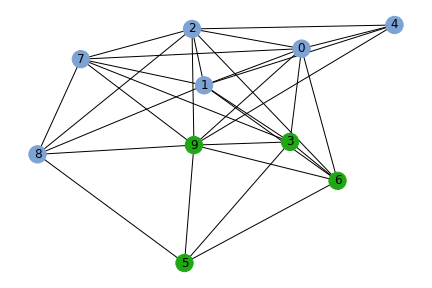
\includegraphics[width=0.9\textwidth]{fig_1.png} % first figure itself
        \caption{\label{fig:fig_1} A visualization of a network with 4 vertices and 4 edges.}
    \end{minipage}\hfill
    \begin{minipage}{0.45\textwidth}
        \centering
        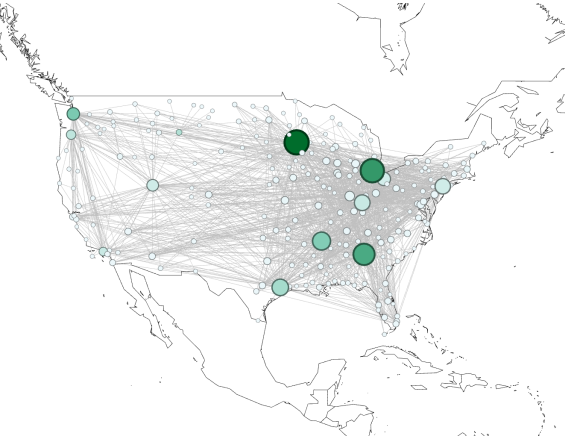
\includegraphics[width=0.9\textwidth]{fig_2.png} % second figure itself
        \caption{\label{fig:fig_2}A network with unique ID and color labels. In this network, there are two communities whose nodes are either colored in sky blue or in grass green.}
    \end{minipage}
\end{figure}


\subsection{Community}

%% (Done)Re-write the remaining part of community section.
%% (Done)Complete Strong/weak community definition
%% (Done)Complete global structure community

In network analysis, community in a network often refers to a group of vertex that has closer relation among each other comparing to other vertices that are not in the same group. For instance, take geographic network for instance with no additional information given, intuitively, let houses be vertices and distance between houses be edges, one may consider vertices that 'cluster' together is more likely to be a community. Of course, there is nothing wrong to determine the formation of community in this way. In fact, if one connect the houses based on the name of the owner, the shape and the scale of the community in the geographic network can be immensely different. Therefore, based on the nature of the network and the properties that researchers are interested in, there is no fix definition of community within network. 

\bigbreak

In general, to express a vertex $v$ is assigned to a community $C_i$, it can be written as $v \in C_i$. Alternatively, in the same scenario, $v$ has a label of $c_i$ and $C_i$ is a collection of vertices that all has a label, $c_i$. Given a partitioned network with n communities, let $C_i$ be the community formed by vertices with a label of $c_i$, if every vertex is assigned to at least one of the community then $\bigcup_{1 \leq i \leq n} C_i \subseteq V(G)$.  Without questioning, a vertex can be partitioned into multiple communities, causing overlapped community. Such phenomena is common in real life networks\cite{2,4,6}. To simplify the complexity of the context, in this dissertation, no vertex will be assigned to multiple communities, that is $\forall C_i,\ C_j \text{, } i \neq j\text{, }C_i \cap C_j = \phi$. 

\bigbreak

In the research \cite{19}, Fortunatoa proposed that a module (community) should contains more edges joining vertices within the same module (intra-community edges) than sum of edges joining vertices across different modules (inter-community edges). The idea is intuitive, the higher density of edges within a sub-graph is more likely to form into a community. Note that as previously mentioned, since network structures analysis can be conducted in various fields; many definitions of community have been characterize by statisticians, physicians, and chemical scientists. In general, community of network can be defined in two ways: One based on the local structure and the other is based on the global structure.

\bigbreak 

\begin{enumerate}[label=(\roman*)]
\item
    Definition of Local Structure: By reading the name, it is not hard to tell that, given a sub-graph of the network that is under examination, the attention is focused on the local structure(sub-graph in this case). Indeed, such definition neglect the influence of the remaining portion other than the sub-graph itself. The local structure definition is mostly used in social network analysis \cite{17} and geographical network analysis \cite{18} since the mutual cohesion within community is often the focus of the studies. The basic evaluation of community is $d_i$, the total degree of the vertex $i$ in network $G$. Degree is the count of edges that connect the vertex to its neighbor vertices. Assume that the network is unweighted and undirected, in terms of adjacency matrix introduced in section 2.1, let $A$ be the adjacency matrix of network $G$, then $d_i = \sum_{j} A_{ij}$. The same expression can be expanded to sub-graph of network. Given a sub-graph, say, $G'$, then 
    
    \begin{equation}\label{eq:com_deg}
    d_i(G') = \sum_{j \in V(G)} A_{ij} = \sum_{(j\in G')} A_{ij} + \sum_{(j\notin G')} A_{ij} = d_i^{in}(G') + d_i^{out}(G').
    \end{equation}
    
    $d_i^{in}(G')$ is the sum of edges that connect vertex $i$ and all other vertices that are within sub-graph $G'$. $d_i^{out}(G')$ is the sum of edges that connect vertex i and all other vertices lies 'outside' of the sub-graph $G'$. 
     
    \bigbreak
     
    By splitting equation\eqref{eq:com_deg} into two components in this fashion, researchers can determine if a sub-graph is indeed a community. Moreover, if a community is successfully identified, the following two definition can indicate if such community is 'strong' or 'weak'.
    
    \begin{enumerate}
        \item Strong Community: Given a sub-graph $G'$, $G'$ is a strong community if
        \begin{equation}\label{eq:strong_com}
        d_i^{in}(G') > d_i^{out}(G'), \forall i \in G'
        \end{equation}
        The strictness of definition of strong community ensures that every nodes within communities has higher intra-community edges than edges connecting the rest of the graph.
        \item Weak Community: Given a sub-graph $G'$, $G'$ is a weak community if
        \begin{equation}\label{eq:weak_com}
        \sum_{i \in G'}d_i^{in}(G') > \sum_{i \in G'}d_i^{out}(G')
        \end{equation}
        By comparing two definitions, it is obvious that weak community only requires the total number of intra-community edges being greater than the total number of inter-community edges.
    \end{enumerate}
    
    Clearly, a strong community can be as well a weak community, but the relation is not mutual, meaning that a weak community may not be a strong community by default. 
    
    For sure, there are additional definitions of community based on varies needs. For instance, k-core is another approach to identify a community that has high similarity to the definition of strong community. A k-core evaluation is that given a sub-graph $G'$, every vertex in $G'$ must have at least k neighbors that are in sub-graph $G'$. Formally, given a subgraph $G'$, $G'$ is a k-core community if 
    
    \begin{equation}\label{eq:k_core}
    d_i^{in}(G') > k, \forall i \in G', k \in N,
    \end{equation}
    where $N$ is the set of natural numbers. Further application of k-core technique can be found in reference \cite{20}.

\item
    Definition of Global Structure: Communities, or so called modules, are basically a fraction of a graph after all. Therefore, it is reasonable to consider the formation of communities in a greater scope. One of the most used method is by comparing network with its null model. The idea of null model is first proposed by Girvan and Newman in reference \cite{8}. A null model of a network shares the same vertex set with the original network, that is to say, the vertex set of null model is equivalent to the set of network. However, as for the edge set of null model, edges within null model are 'rewired' randomly; the rewiring process can be achieved by applying Maslov-Sneppen rewiring algorithm\cite{22}. Since edges of null model do not follow properties that may hold in the original network yet follows the randomness of some distribution, null model does not, or at least as no intention to, reveal traits of community structure in general cases. [It is worth mentioning that due to the nature of current randomness generating algorithms, computers nowadays are not capable of producing true random distributions for constructing null models, further study can be found in \cite{21, 22}.] By implementing null model to compare with the structure, the result of comparison can illustrate the existence of communities and exhibit their size and their characteristics.

\end{enumerate}


Depending on the content of network, such as social network, chemical network, and ecosystem network, the definition of a community may vary. In fact, in numerous community detection algorithms, definitions of community are often byproducts of the algorithms to evaluate if the current partition requires further optimization \cite{19}. Additionally, if given a weighted network such as a geographical network, we can intuitively determine if vertices can be grouped into a community by taking their distance(weight of edges) into consideration. Directed network can also be partitioned into communities if the community detection is designed carefully with the help of linear algebra and information theory\cite{4}. As mentioned previously, there are networks that has no intention of creating communities such as random graphs or Barabási–Albert model\cite{5}; researchers can still apply community detection algorithms to unveil latent structure from these random graphs yet the interpretation of such results can be impractical.

\pagebreak

\section{Goodness of Partition}

Intuitively, to examine if a partition is 'good' or not, researchers should measure following two properties: 
\begin{enumerate}[label=(\alph*)]
\item Tightness: Vertices within the same community should have strong relation.
\item Sparsity: Communities should have weak relation mutually.
\end{enumerate}

In this section, a number of approaches will be introduced to evaluate the partition considering the properties mentioned above. Other additional properties such as betweeness, conductivity, and modularity are often take into consideration for better understanding of specific types of real-world network\cite{7,8}; some advanced properties will also be explained in this section.

\subsection{Performance Evaluation}
A good partition should have high tightness intra-community-wise and strong trait of sparsity inter-community-wise. Given a undirected partitioned network, a performance function $P(G)$ is defined as
$$P(G) = \frac{\text{edge of intra-community} + \text{non-edge of inter-community}}{\text{total potential edges}}
$$
$$
=\frac{|E_{intra}| + [n*(n-1) - |E_{intra}| - |E_{inter}|]}{n*(n-1)/2}
$$
\begin{equation}\label{eq:perf_eva3}
=2*\left[ 1 - \frac{ |E_{inter}| } { n*\left( n-1 \right) }  \right],
\end{equation}
where G is a partitioned network, $E_{intra}$ is the set of edges lie within communities, $E_{inter}$ is the set of edges connecting vertices between two different communities. 

\bigbreak

After a series of rearrangement, it is not difficult to observe that a network has smaller set of inter-community edges can leads to higher value of $P(G)$, which indicates better performance\cite{7}. In the aspect of algorithm complexity analysis, the time complexity of performance evaluation is in $O(E)$, where E is the edge set; with linear time complexity, researchers can conduct faster initial evaluation comparing to other advanced evaluation procedures. 

\subsection{Mean Square Error}
For networks with coordinates provided, take geographical network or cosmic network for instance \cite{9,10}, computing the mean square error(MSE) evaluation can give us an idea if a partition is good. A demonstration of geographical network is shown in figure \ref{fig:fig_3}. The quality function of MSE evaluation is defined as follows:
\begin{equation}\label{MSE1}
	Q(G) = \sum_{i}^{k}\sum_{j}^{n} M_{i j} * |v_{j} - \bar{v}_{i}|^{2},
\end{equation}
   
where G is a partitioned network, k is the total number of communities in a partition, n is the count of the vertices of network $G$, $M$ is a k by n communities matrix, 
\[
      M_{ij} = 
      \begin{cases}
        1, &  v_{j} \in C_i\\
        0, & \text{otherwise}
      \end{cases}
\]

, and $\bar{v}_{i}$ is the arithmetic center of $C_i$. 

\bigbreak

This evaluation is relatively straightforward; given a well-partitioned network, it is expected that vertices within the same community cluster densely and surround the center of the community; such behavior results in mean square error within every community should be relatively small. What's more is that the idea computing the euclidean distance between vertices (or so called $l_2$ norms)  as part of community evaluation is not uncommon in network analysis. k-cluster is an algorithm partitioning network into clusters(communities); k-cluster first iterate through every vertices,  cluster the k amount of nearest neighbors into the same cluster by computing the distance between every other vertices and the chosen vertex, re-iterate the remaining vertices that are not clustered, and eventually stop the algorithm if there is no progress of partitioning. As for the aspect of computational expense, assume calculating the distance between vertices takes constant time, the computation complexity of MSE evaluation is in $O(C*V)$, where $C$ is the number of communities within network and $V$ is the vertex set of network, the computing time can be reduced by pre-allocating vertices into a collection of set distributed by the partition.

\begin{figure}
\centering
\includegraphics[width=0.6\textwidth]{fig_3.png}

\caption{\label{fig:fig_3}An airline flight network of the United States of America\cite{11}.}
\end{figure}

\subsection{Modularity}

This evaluation method is first introduced by Blondel in 2008 \cite{12}. When tackling with a humongous and complex network, a fast and approximated evaluation algorithm is necessary for time and resource efficiency. In this end, the modularity evaluation stands out to do this job. The modularity function \cite{13} can be written as follows:
\begin{equation}\label{eq:modularity}
Q = \sum_{i=1}^c \left[  \frac{e_i}{m} - \left( \frac{deg_i}{2m} \right)^2  \right],
\end{equation}
where $c$ is the count of communities, $e_i$ is the count of edges within the community $i$, $m$ is the count of the edge of the network, and $deg_i$ is the total degree of vertices within community $i$. The logic of modularity is similar to hypothesis testing: an alternative model and a null model is defined for comparison. The first term of equation \eqref{eq:modularity}, which is the alternative model in this case, is the fraction of edges within a community to total edges of the network; and the second term, the null model, is the expected fraction based on the assumption that edges are randomly connected.

\bigbreak

Given an undirected and unweighted network, the value of modularity lies in range $[-1, 1]$. If the edges within a community exceed the expected count of edges, the first term will be greater than the second term, leading the $Q$ value of that community become positive. This implies that the edges inside the community are averagely concentrated. As author stated in the original paper \cite{12}, implementing modularity to examine the partition is not the only usage. The modularity function is as well suitable for partition optimization for  networks. The community detection algorithms that import modularity optimization, such as Louvain method, will be discussed in the latter section.

\bigbreak

Despite the time complexity of computing modularity is in $O(n*log n)$, which is faster comparing to other meta partition evaluations \cite{2, 12}, the modularity evaluation is not capable of detecting small communities. The defect is inevitable due to the nature of the null model defined previously, the modularity only considers the structure of communities under global scope; as for local structure evaluation, the modularity ignores heterogeneity of sizes between communities \cite{13}. In real world applications \cite{9, 10}, the modularity evaluation may suggest small communities should be merged into a greater community, causing false estimation of structure and count of communities. Such over-merging behavior is called resolution limit \cite{13}.

%% (Done)Read more about modularity and it's concept
%% (Done)Read resolution limit (over-merging) 

\subsection{Normalized Mutual Information}

%%(Done, but not related) Read Community Structure - Section 6
%% (Done)Work on NMI chapter intro
%% (Done)In Evaluation of Community Detection Methods, NMI is counter-intuitive and unreasonable due to lack of consideration of local community strucure
%% (Done)Introduce new NMI indicator: adding the summation of v_partition/v_true as coefficients into orginal NMI model(Treat all communities equally to reduce size discrepancy)
%% (Done)Read page 3 "Evaluation of Community Detection Methods"

Despite previous approaches have proven their functionality in may applications, yet there is lack of consideration of 'real' partitions. A real partitions, or so called ground-truth labels, are networks that already have labels for evaluation. In this sub-section, the normalized mutual information(NMI) takes the ground-truth labels into partition evaluation. The idea of normalized mutual information in network analysis is derived from entropy computation in information theory. The original usage of NMI is similar to NMI is information theory: a measurement to determine the quality of cluster\cite{23}. 

The calculation of mutual information is identical to it in information theory. Given a discrete random variable $X$, the entropy of $X$ is defined as:

\begin{equation}\label{eq:mi1}
H(X) = - \sum_{x\in X} p(x)  log(p(x)),
\end{equation}where $p(x)$ is the probability of x.
\bigbreak
By extending the context of  formula \ref{eq:mi1}, we can define the joint entropy of $X$ and another discrete random variable Y as:
\begin{equation}\label{eq:mi2}
H(X, Y) = - \sum_{x\in X} \sum_{y \in Y} p(x, y)  log(p(x, y)).
\end{equation}
\bigbreak
Similarly,  the conditional entropy of X with given Y is as follows:
\begin{equation}\label{eq:mi3}
H(X|Y) = -\sum_{x \in X} p(x) H(x|y) = -\sum_{x \in X}\sum_{y \in Y} p(x,y) log(p(x|y)).
\end{equation}
With the above definitions of entropy, joint entropy, and conditional entropy, the mutual information can be finally defined as follows:

\begin{equation}\label{eq:mi4}
I(X;Y) = H(X) - H(X|Y)
\end{equation}

The intuition of mutual information is to calculate of similarity between the partition one would like to investigate and the ground-truth partition. The visualization of the relation among types of entropy are shown in figure \ref{fig:fig_4}. By now, it is obvious that the purpose of mutual information measurement matches our intention to evaluate the partition considering ground-truth partition. However, since the value of mutual information of two partitions can be any non-negative number, it is difficult to interpret the result solely be reading the value of it. Hence, a normalization of mutual information is necessary to improve the interpretability. Therefore, the NMI can be defined as follows:

\begin{equation}\label{eq:nmi}
NMI(X;Y) = \frac{2*I(X; Y)}{H(X,Y) + I(X;Y)}.
\end{equation}

\begin{figure}
\centering
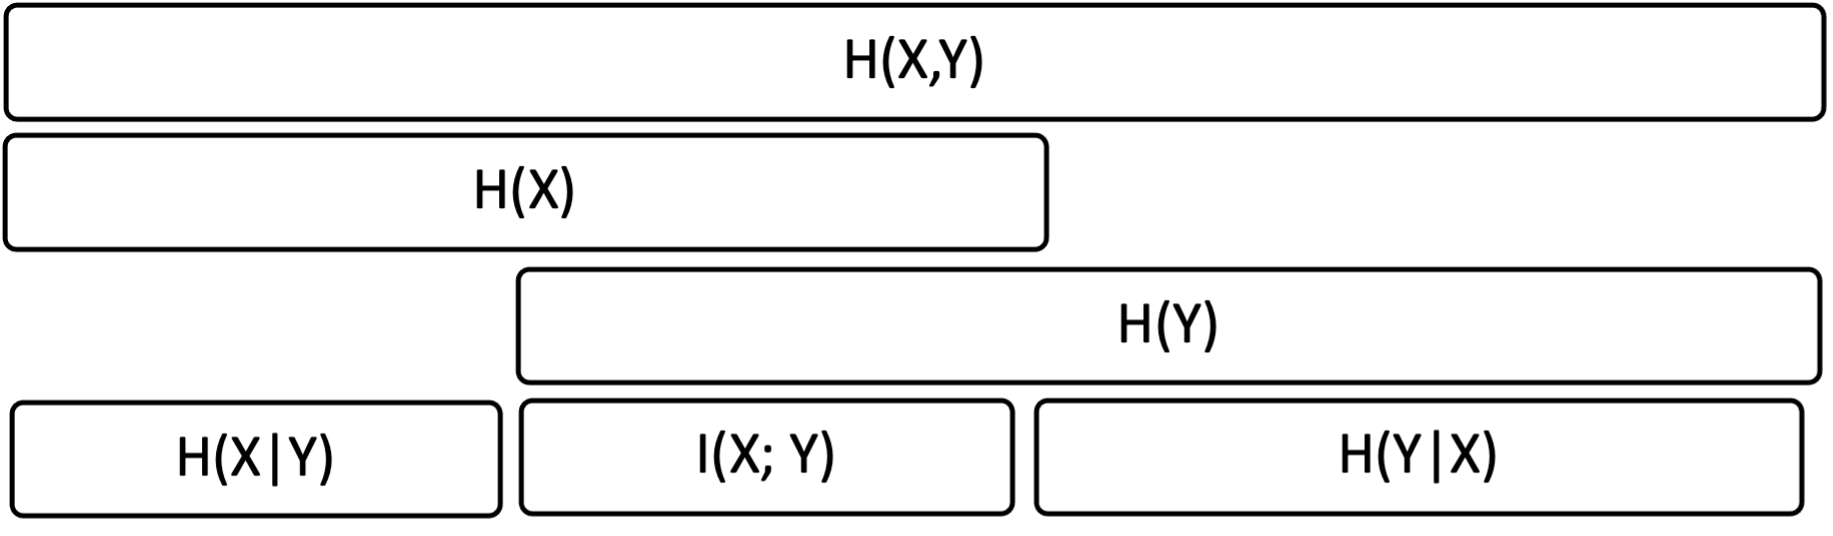
\includegraphics[width=0.6\textwidth]{fig_4.png}

\caption{\label{fig:fig_4}The visualization of relation among joint entropy, conditional entropy, and mutual information.}
\end{figure}
%% (Done)Continue working on NMI, read the procedure of Evaluation of Community Detection Methods, Page 3, below equation 13
By normalizing mutual information, NMI is bounded between 0 (no correlation) and 1 (perfect correlation) inclusively, which helps researchers to interpret the result. However, due to the nature of normalized mutual information, the calculation of entropy requires approximation of  probability between ground-truth label and partition; the approximation of probability is often done by calculating the frequency, this leads to finite size effect\cite{10}. A finite size effect is that the interest of research is not independent to the size of the model, which can be disadvantageous when analysis needs to be done under size-independent circumstances.

\bigbreak

Moreover, despite normalized mutual information is able to notice the importance of small communities to a certain degree unlike the evaluation by modularity discussed in the previous sub-section, the normalized mutual information may sometimes leads to counter-intuitive result. For instance, say, a network with provided ground-truth labels, (1, 1, 1, 1, 1, 2, 2, 2, 3, 3), the order of labels is determined by the ID of vertices. [Note that the order is irrelevant to the calculation of NMI due to the nature of this evaluation method.] Given two partitions, A = (1, 1, 1, 1, 2, 2, 2, 2, 3, 3) and B = (1, 1, 1, 1, 1, 2, 2, 2, 2, 3), by visually comparing two partitions, one can intuitively conclude that partition A has higher similarity to the ground-truth label than partition B does since in partition A, community of label 3 is preserved and only a small portion of community with label 1 are effected . Nonetheless, the normalized mutual information of partition A and partition B is 0.77 and 0.81, indicating that partition B has better correlation to the ground-truth label than partition A does, which is counter-intuitive.

\bigbreak

The time complexity of normalized mutual information is in $O(n^2)$, where $n$ is the number of vertices in the network. The quadratic time complexity can be problematic and time consuming if applied on large complex network. Since NMI focuses on the distribution of cluster instead of the structure between edges and vertices, NMI outperforms other evaluation methods if $E(G) >>V(G)$
, where E(G) is the edge set of network G and V(G) is the vertex set of network G.

\subsection{Adaptive Mutual Information}
%%Patches to NMI to encourage the completeness of community no matter the size of the community.

%% Discuss the properties of the scale_check function and how the function performs in different sizes

\pagebreak
\begin{thebibliography}{100}

\bibitem{1}
  
    \textit{Community detection algorithms: A comparative analysis},
    Lancichinetti, A. and Fortunato, S.,2009.
    1986.
  
\bibitem{2}
    \textit{Parallel Protein Community Detection in
    Large-scale PPI Networks Based on
    Multi-source Learning}
    J. Chen, K. Li, K. Bilal, A. A. Metwally, K. Li, and P. S. Yu,
    2018
    
\bibitem{3}
    \textit{Community detection in Social Media. Data Mining and Knowledge Discovery}
    Papadopoulos, S., Kompatsiaris, Y., Vakali, A. and Spyridonos, P.,
    2011
    
\bibitem{4}
    \textit{Quantitative methods for ecological network analysis. Computational Biology and Chemistry}
    Ulanowicz, R.E.,
    2004
    
\bibitem{5}
    \textit{tatistical mechanics of complex networks. Reviews of Modern Physics}
    Albert, R. and Barabási, A.-L.,
    2002
    
\bibitem{6}
    \textit{Comparison of Graph Databases and Relational Databases When Handling Large-Scale Social Data}
    Chen, Yaowen,
    2016
    
\bibitem{7}
    \textit{Community detection in graphs}
    Fortunato, S.,
    2010
    
\bibitem{8}
    \textit{Community structure in social and biological networks}
    Girvan, M. and Newman, M.E.J.,
    2002
    
\bibitem{9}
    \textit{Network analysis of the COSMOS galaxy field}
    de Regt, R., Apunevych, S., von Ferber, C., Holovatch, Y. and Novosyadlyj, B,
    2018
    
\bibitem{10}
    \textit{Evaluation of Community Detection Methods}
    Liu, X., Cheng, H.-M. and Zhang, Z.-Y,
    2019
    
\bibitem{11}
    \textit{An Introduction of Gephi}
    2017

\bibitem{12}
    \textit{Fast unfolding of communities in large networks}
    Blondel, V.D., Guillaume, J.-L., Lambiotte, R. and Lefebvre, E
    2008
    
\bibitem{13}
    \textit{Resolution limit in community detection}
    Fortunato, S. and Barthelemy, M.,
    2006

\bibitem{14}
	{Federal-Aid Highway Act of 1956: Creating The Interstate System}
	Richard F. Weingroff,
    1996
    
   \bibitem{15}
   	{Introduction to Graph Theory Fourth edition }
    Robin J. Wilson,
    1996
    
    \bibitem{16}
    {Role of Adjacency Matrix & Adjacency List in Graph Theory}
    Harmanjit S., Richa S.,
    2012
        
    \bibitem{17}
    {Models and Methods in Social Network Analysis}
    Carrington, P.J., Scott, J. and Wasserman, S.,
    2005
    
    \bibitem{18}
    {Geographical Network Analysis}
    Uitermark, J. and Meeteren, M.,
    2021
    
    \bibitem{19}
    {Community Structure in Graphs}
    Santo Fortunatoa, Claudio Castellanob,
    2007
    
    \bibitem{20}
    {s-core network decomposition: A generalization of k-core analysis to weighted networks}
    Eidsaa, M. and Almaas, E.,
    2013
    
    \bibitem{21}
    {MIT School of Engineering |» Can a computer generate a truly random number? [online] Mit Engineering}
    Rubin, J.,
    2011
    
    \bibitem{22}
    {Null Models of Economic Networks: The Case of the World Trade Web}
    Giorgio Fagiolo · Tiziano Squartini · Diego Garlaschelli,
    2012
    
    \bibitem{23}
    {On Normalized Mutual Information: Measure Derivations and Properties}
    Tarald Kvalseth,
    2017
    
\end{thebibliography}

\end{document}